\documentclass[12pt]{article}
\usepackage{xcolor}
\usepackage{amsmath}
\usepackage{tikz}

\begin{document}

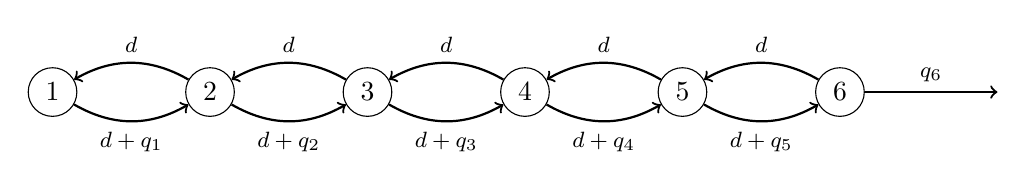
\begin{tikzpicture}
\begin{scope}[every node/.style={draw}, node distance= 1.5 cm]
    \node[circle] (1) at (0,0) {$1$};
    \node[circle] (2) at (2,0) {$2$};
    \node[circle] (3) at (4,0) {$3$};
    \node[circle] (4) at (6,0) {$4$};

    \node[circle] (5) at (8,0) {$5$};
    \node[circle] (6) at (10,0) {$6$};
\end{scope}
\begin{scope}[every node/.style={fill=white},
              every edge/.style={thick}]
    \draw[thick] [->](1) to [bend right] node[below=0.1] {{\footnotesize $d+q_1$}} (2);
    \draw[thick] [->](2) to [bend right] node[below=0.1] {{\footnotesize $d+q_2$}} (3);
    \draw[thick] [->](3) to [bend right] node[below=0.1] {{\footnotesize $d+q_3$}} (4);
    \draw[thick] [->](4) to [bend right] node[below=0.1] {{\footnotesize $d+q_4$}} (5);
    \draw[thick] [->](5) to [bend right] node[below=0.1] {{\footnotesize $d+q_5$}} (6);
    \draw[thick] [<-](1) to [bend left] node[above=0.1] {{\footnotesize $d$}} (2);
    \draw[thick] [<-](2) to [bend left] node[above=0.1] {{\footnotesize $d$}} (3);
    \draw[thick] [<-](3) to [bend left] node[above=0.1] {{\footnotesize $d$}} (4);
    \draw[thick] [<-](4) to [bend left] node[above=0.1] {{\footnotesize $d$}} (5);
    \draw[thick] [<-](5) to [bend left] node[above=0.1] {{\footnotesize $d$}} (6);
    \draw[thick] [->](6) to  node[above=0.1] {{\footnotesize $q_6$}} (12, 0);
\end{scope}
\end{tikzpicture}

\end{document}